\documentclass[xcolor={usenames,dvipsnames,svgnames,table}]{beamer}

%Load the myriad packages
\usepackage[orientation=landscape,size=a0,scale=1.4]{beamerposter}

% load macros and prevent authblk from loading
\makeatletter
% prevent a package from loading
\newcommand{\dontusepackage}[2][]{%
    \@namedef{ver@#2.sty}{9999/12/31}%
    \@namedef{opt@#2.sty}{#1}
}

% a macro to load packages only if they are not yet loaded, needed for combination of beamer and hyperref
\newcommand{\usepackagesave}[2][{}]{
    \ltx@ifpackageloaded{#2}{}{
        \usepackage[#1]{#2}}
}
\makeatother
\dontusepackage{authblk}

% load packages, settings and definitions
% this file contains all commonly used packages for the Rattlesnake documentation
% new package, add comment what they are used for

% command packages
\usepackage{xifthen}     % if -then else command

% language and font improvements
\usepackage[english]{babel}	% Multilingual support - https://www.ctan.org/pkg/babel
\usepackage[utf8]{inputenc} % Accept different input encodings - https://www.ctan.org/pkg/inputenc
\usepackage[kerning,spacing,babel]{microtype} % Subliminal refinements towards typographical perfection - https://www.ctan.org/pkg/microtype
\usepackage{eepic}      % Extensions to epic - https://www.ctan.org/pkg/eepic
\usepackage{epic}       % Enhance LaTeX picture mode - https://www.ctan.org/pkg/epic
\usepackage[T1]{fontenc} % selecting font encodingsselecting font encodings - https://www.ctan.org/pkg/fontenc
\usepackage{lmodern}

% title packages
\usepackage{authblk}		% footnote style author/affiliation - https://www.ctan.org/pkg/authblk

% symbols
\usepackage{upgreek}		% Upright Greek letters - https://www.ctan.org/pkg/upgreek
\usepackage{cancel}			% \cancel cmd - https://www.ctan.org/pkg/cancel

% chemical and isotope packages
\usepackage{isotope}		% isotope command - https://www.ctan.org/pkg/isotope
%\usepackage{mhchem}			% chemical formulae/equations - https://www.ctan.org/pkg/mhchem

% layout packages
\usepackage{xspace}			% smart space \xspace - https://www.ctan.org/pkg/xspace
\usepackage{icomma}			% smart math comma - https://www.ctan.org/pkg/icomma
\usepackage{chngpage}		% page layout change during document - https://www.ctan.org/pkg/chngpage
\usepackage[usenames,dvipsnames,svgnames,table]{xcolor}			% color definitions - https://www.ctan.org/pkg/xcolor
\usepackage{enumitem}   % layout for itemize and enumerate - http://www.ctan.org/pkg/enumitem
\usepackage{setspace}    % allows for \singlespacing, \onehalfspacing, and \doublespacing commands - https://www.ctan.org/pkg/setspace

% floating packages
% needed by the breakalgo environment labelsep=quad
\usepackage[singlelinecheck=false, labelsep=quad]{caption}	% table captions - https://www.ctan.org/pkg/caption
\usepackage{subcaption}		% Support for sub-captions - https://www.ctan.org/pkg/subcaption
\usepackage{placeins}   	% Control float placement - https://www.ctan.org/pkg/placeins
\usepackage{float}      	% Improved interface for floating objects - https://www.ctan.org/pkg/float

% table packages
\usepackage{supertabular}	% multi-page tables package - https://www.ctan.org/pkg/supertabular
\usepackage{booktabs}		% table settings - https://www.ctan.org/pkg/booktabs
\usepackage{array}			% Extending the array and tabular environments - https://www.ctan.org/pkg/array
\usepackage{multirow}		% tabular cells spanning multiple rows - https://www.ctan.org/pkg/multirow
% \usepackage{tabls}      % Better vertical spacing in tables and arrays - https://www.ctan.org/pkg/tabls
\usepackage{colortbl}      % Allows for color manipulation within tables - https://www.ctan.org/pkg/colortbl

% pictures, plots and listings
\usepackage{graphicx}		% include graphics - https://www.ctan.org/pkg/graphicx
\usepackage{wrapfig}		% wrapfigure enviroment - https://www.ctan.org/pkg/wrapfig
\usepackage{pgfplots}		% latex plots - https://www.ctan.org/pkg/pgfplots


% source code and algorithms
\usepackage{algorithmicx} % newer version of algorithmic - https://www.ctan.org/pkg/algorithmicx
\usepackage{listings} 	% source code listings - http://www.ctan.org/pkg/listings
\usepackage{verbatim}   % verbatim - https://www.ctan.org/pkg/verbatim

% misc packages
\usepackage{url}        % provide \url command for web addresses - https://www.ctan.org/pkg/url
\usepackage{import}			% Establish input relative to a directory - https://www.ctan.org/pkg/import
\usepackage{afterpage}  % Execute command after the next page break - https://www.ctan.org/pkg/afterpage
\usepackage{lscape}     % Place selected parts of a document in landscape - https://www.ctan.org/pkg/lscape
\usepackage{rotating}   % Rotation tools, including rotated full-page floats - https://www.ctan.org/pkg/rotating
\usepackage{chngcntr}   % Change the resetting of counters - http://ctan.org/pkg/chngcntr
\usepackage{textpos}    % Allows logo and banner manipulation

% eps support
\usepackage{epsfig}       % include eps figures - https://www.ctan.org/pkg/epsfig
\usepackage{epsf}          % Simple macros for EPS inclusion - https://www.ctan.org/pkg/epsf
\usepackage{epstopdf}   %use .eps images (as pdf) in \includegraphics


% reference packages
% hyperref must be loaded before amsmath to avoid problems with subequations and align
\usepackage{hyperref}		% Extensive support for hypertext - https://www.ctan.org/pkg/hyperref


% packages that must be loaded after hyperref - http://tex.stackexchange.com/questions/1863/which-packages-should-be-loaded-after-hyperref-instead-of-before
\usepackage{geometry}		% Flexible and complete interface to document dimensions - https://www.ctan.org/pkg/geometry
\usepackage{algorithm}  % algorithm enviroment

% ams math packages
\usepackage{amsmath}    % mathematical facilities - https://www.ctan.org/pkg/amsmath
\usepackage{amsfonts}   % fonts for math - https://www.ctan.org/pkg/amsfonts
\usepackage{amssymb}    %
\usepackage{amsthm}     % Typesetting theorems - https://www.ctan.org/pkg/amsthm

\usepackage{nameref}		% allows references with names instread of numbers \nameref - http://www.ctan.org/pkg/nameref
\usepackage[capitalize,nameinlink]{cleveref}   % smart references - http://ctan.org/pkg/cleveref

\usepackage{exscale} 		% needs to stay at the end of package loading to fix integral signs
% general settings
\renewcommand\floatpagefraction{0.75} % threshold for floating objects to be placed on a page

\makeatletter
% center floats generally
\g@addto@macro\@floatboxreset\centering
% gives the current section name
\newcommand*{\currentname}{\@currentlabelname}
\makeatother

% figure setting, controlles the height of pgfplots from the main script
\newlength{\figheight}
\setlength{\figheight}{12cm}

% example for hyperref setup, we have to see if we can get that better
\hypersetup{
  linktocpage=true,       % links in table of contents
  bookmarks=true,         % show bookmarks bar?
  unicode=true,           % non-Latin characters in Acrobat's bookmarks
  pdftoolbar=true,        % show Acrobat's toolbar?
  pdfmenubar=true,        % show Acrobat's menu?
  pdffitwindow=false,     % window fit to page when opened
  pdfstartview={FitH},    % fits the width of the page to the window
  pdfnewwindow=true,      % links in new window
  colorlinks=false,       % false: boxed links; true: colored links
  linkcolor=red,          % color of internal links
  citecolor=green,        % color of links to bibliography
  filecolor=magenta,      % color of file links
  urlcolor=cyan,          % color of external links
  pdfborder={0 0 0},      % color of link frames
}


% set package versions
\pgfplotsset{compat=1.12}

% set table and figure counters here

% set up listings - see https://en.wikibooks.org/wiki/LaTeX/Source_Code_Listings
\lstset{ %
  backgroundcolor=\color{white},   % choose the background color; you must add \usepackage{color} or \usepackage{xcolor}; should come as last argument
  basicstyle=\footnotesize,        % the size of the fonts that are used for the code
  breakatwhitespace=false,         % sets if automatic breaks should only happen at whitespace
  breaklines=true,                 % sets automatic line breaking
  captionpos=b,                    % sets the caption-position to bottom
  commentstyle=\color{Gray},       % comment style
  deletekeywords={...},            % if you want to delete keywords from the given language
  escapeinside={\%*}{*)},          % if you want to add LaTeX within your code
  extendedchars=true,              % lets you use non-ASCII characters; for 8-bits encodings only, does not work with UTF-8
  frame=single,	                   % adds a frame around the code
  keepspaces=true,                 % keeps spaces in text, useful for keeping indentation of code (possibly needs columns=flexible)
  keywordstyle=\color{blue},       % keyword style
  morekeywords={*,...},            % if you want to add more keywords to the set
  numbers=left,                    % where to put the line-numbers; possible values are (none, left, right)
  numbersep=5pt,                   % how far the line-numbers are from the code
  numberstyle=\tiny\color{Gray},   % the style that is used for the line-numbers
  rulecolor=\color{black},         % if not set, the frame-color may be changed on line-breaks within not-black text (e.g. comments (green here))
  showspaces=false,                % show spaces everywhere adding particular underscores; it overrides 'showstringspaces'
  showstringspaces=false,          % underline spaces within strings only
  showtabs=false,                  % show tabs within strings adding particular underscores
  stepnumber=2,                    % the step between two line-numbers. If it's 1, each line will be numbered
  stringstyle=\color{mymauve},     % string literal style
  tabsize=2,	                     % sets default tabsize to 2 spaces
  title=\lstname                   % show the filename of files included with \lstinputlisting; also try caption instead of title
}

% define style for moose
\lstdefinestyle{cpp}{
  belowcaptionskip=1\baselineskip,
  breaklines=true,
  frame=TB,
  xleftmargin=\parindent,
  language=C,
  showstringspaces=false,
  basicstyle=\footnotesize\ttfamily,
  keywordstyle=\bfseries\color{green!40!black},
  commentstyle=\itshape\color{purple!40!black},
  identifierstyle=\color{blue},
  stringstyle=\color{orange},
}

\lstdefinestyle{python}{
  belowcaptionskip=1\baselineskip,
  breaklines=true,
  frame=,
  xleftmargin=\parindent,
  language=Python,
  showstringspaces=false,
  basicstyle=\footnotesize\ttfamily,
  keywordstyle=\bfseries\color{blue},
  commentstyle=\itshape\color{gray},
  identifierstyle=\color{black},
  stringstyle=\color{green},
}

\lstdefinelanguage{Moose}{
  morekeywords={one,two,three,four,five,six,seven,eight,
  nine,ten,eleven,twelve,o,clock,rock,around,the,tonight},
  sensitive=false,
  morecomment=[l]{//},
  morecomment=[s]{/*}{*/},
  morestring=[b]",
}

\lstdefinestyle{moose}{
  belowcaptionskip=1\baselineskip,
  breaklines=true,
  frame=tb,
  xleftmargin=\parindent,
  language=Moose,
  showstringspaces=false,
  basicstyle=\footnotesize\ttfamily,
  keywordstyle=\bfseries\color{blue},
  commentstyle=\itshape\color{gray},
  identifierstyle=\color{black},
  stringstyle=\color{green},
}

\lstset{literate=
  {á}{{\'a}}1 {é}{{\'e}}1 {í}{{\'i}}1 {ó}{{\'o}}1 {ú}{{\'u}}1
  {Á}{{\'A}}1 {É}{{\'E}}1 {Í}{{\'I}}1 {Ó}{{\'O}}1 {Ú}{{\'U}}1
  {à}{{\`a}}1 {è}{{\`e}}1 {ì}{{\`i}}1 {ò}{{\`o}}1 {ù}{{\`u}}1
  {À}{{\`A}}1 {È}{{\'E}}1 {Ì}{{\`I}}1 {Ò}{{\`O}}1 {Ù}{{\`U}}1
  {ä}{{\"a}}1 {ë}{{\"e}}1 {ï}{{\"i}}1 {ö}{{\"o}}1 {ü}{{\"u}}1
  {Ä}{{\"A}}1 {Ë}{{\"E}}1 {Ï}{{\"I}}1 {Ö}{{\"O}}1 {Ü}{{\"U}}1
  {â}{{\^a}}1 {ê}{{\^e}}1 {î}{{\^i}}1 {ô}{{\^o}}1 {û}{{\^u}}1
  {Â}{{\^A}}1 {Ê}{{\^E}}1 {Î}{{\^I}}1 {Ô}{{\^O}}1 {Û}{{\^U}}1
  {œ}{{\oe}}1 {Œ}{{\OE}}1 {æ}{{\ae}}1 {Æ}{{\AE}}1 {ß}{{\ss}}1
  {ű}{{\H{u}}}1 {Ű}{{\H{U}}}1 {ő}{{\H{o}}}1 {Ő}{{\H{O}}}1
  {ç}{{\c c}}1 {Ç}{{\c C}}1 {ø}{{\o}}1 {å}{{\r a}}1 {Å}{{\r A}}1
  {€}{{\euro}}1 {£}{{\pounds}}1
}

% Common style and macro defintions for CLASS documents
%=================================================================================================

%%% General Commands

%% structural elements
% An explanation for a function
\newcommand{\explain}[1]{\mbox{\hspace{2em} #1}}
% attemtion box
\newcommand{\attention}[1]{\mbox{\hspace{2em} #1}}
% comments at the sde of the paragraph
\newcommand{\sidenotes}[1]{\marginpar{ {\footnotesize #1} }}
% create empty double page, TODO do we need that?
\newcommand{\clearemptydoublepage}{\newpage{\pagestyle{empty}\cleardoublepage}}
%TODO description here
\newcommand{\apost}{\textit{a posteriori\xspace}}
%TODO description here
\newcommand{\Apost}{\textit{A posteriori}\xspace}

%%% Math
%% Paratnhis etc.
% ()
\newcommand{\parenthesis}[1]{{\left(#1 \right)}}
% []
\newcommand{\bracket}[1]{{\left[ #1 \right]}}
% {}
\newcommand{\bracet}[1]{{\left\{#1 \right\}}}
% <>
\newcommand{\angled}[1]{{\left\langle#1\right\rangle}}

%% common math symbols
% imaginary number
\newcommand{\img}{\ensuremath{\hat{\imath}}\xspace}
% gradient symbol
\newcommand{\grad}{\vec{\nabla}}
\newcommand{\del}{\vec{\nabla}}
% adjoint
\newcommand{\adj}[2][{}]{{{#2}^{\dagger#1}}}
% order number
\newcommand{\order}[1]{^\parenthesis{#1}}
% iteration number
\newcommand{\iter}[1]{^{#1}}

%% common math function
% divergence
\renewcommand{\div}{\del\! \cdot \!}
% rotation
\newcommand{\rot}{\del\! \times \!}
% absolute value
\newcommand{\abs}[1]{\left|#1\right|}
% norm
\newcommand{\norm}[2][{}]{\lVert#2\rVert_{#1}}
% e function
\newcommand{\e}[1]{\mathrm{e}^{#1}}
% power of ten
\newcommand{\tento}[1]{\ensuremath{10^{#1}}\xspace}
% E notation
\newcommand{\E}[1]{\ensuremath{\cdot \tento{#1}}\xspace}
% sign
\DeclareMathOperator{\sign}{sign}

%% fraction
% 1 / 2
\newcommand{\half}[1][1]{\frac{#1}{2}}
% 1 / 3
\newcommand{\third}[1][1]{\frac{#1}{3}}
% 1 / 4
\newcommand{\fourth}[1][1]{\frac{#1}{4}}

% vectors etc
% vector, we use standard latex notation
% matrix
\newcommand{\mat}[1]{\mathbf{#1}}
% tensor
\newcommand{\tensor}[1]{\underline{\underline{#1}}}
% operator symbol
\newcommand{\op}[1]{\mathrm{\mathbf{#1}}}

% derivatives
% first derivatives
% general first derivative, with optional argument for f
\newcommand{\dd}[2][]{\frac{\partial #1}{\partial #2}}
% partial derivative for x, optional argument for f
\newcommand{\ddx}[1][]{\dd[#1]{x}}
% partial derivative for y, optional argument for f
\newcommand{\ddy}[1][]{\dd[#1]{y}}
% partial derivative for z, optional argument for f
\newcommand{\ddz}[1][]{\dd[#1]{z}}
% partial derivative for t, optional argument for f
\newcommand{\ddt}[1][]{\dd[#1]{t}}

% second derivatives, only for a single variable, cross derivatives are too many
% second general derivative, optional argument for f
\newcommand{\ddd}[2][{}]{\frac{\partial^2 #1}{\partial {#2}^2}}
% second partial derivative for x, optional argument for f
\newcommand{\ddxx}[1][]{\ddd[#1]{x}}
% second partial derivative for y, optional argument for f
\newcommand{\ddyy}[1][]{\ddd[#1]{y}}
% second partial derivative for z, optional argument for f
\newcommand{\ddzz}[1][]{\ddd[#1]{z}}
% second partial derivative for t, optional argument for f
\newcommand{\ddtt}[1][]{\ddd[#1]{t}}

% integrals
% integral dx, optional parameter for different variable
\newcommand{\dx}[1][x]{\,d#1}
% integral dy
\newcommand{\dy}{\dx[y]}
% integral dz
\newcommand{\dz}{\dx[z]}
% integral dt
\newcommand{\dt}{\dx[t]}
%integral dmu
\newcommand{\dmu}{\dx[\mu]}
%integral dOmega
\newcommand{\domg}{\dx[\direction]}

% spherical integrals
% shortcut for sphere notation
\newcommand{\sphere}{\ensuremath{\mathcal{S}}\xspace}
% angular quadrature weight
\newcommand{\aqweight}{\omega}

% integral over full sphere
\newcommand{\intsp}{\int_{4\pi}}
% integral over half sphere
\newcommand{\inthalfsp}{\int_{2\pi}}
% polar integral
\newcommand{\intpolar}{\int_{-1}^{1}}
% negative partial polar integral
\newcommand{\intnpolar}{\int_{-1}^{0}}
% positive partial polar integral
\newcommand{\intppolar}{\int_{0}^{1}}


% FEM symbols
% spatial domain
\newcommand*{\domain}{\ensuremath{\mathcal{D}}\xspace}
% boundary of a spatical domain
\newcommand*{\boundary}{\ensuremath{{\partial\domain}}\xspace}
% vacuum boundary of a spatical domain
\newcommand*{\vboundary}{\ensuremath{{\boundary}_v}\xspace}
% reflective boundary of a spatical domain
\newcommand*{\rboundary}{\ensuremath{{\boundary}_r}\xspace}
% interface surface
\newcommand*{\interface}{\ensuremath{{\Gamma}}\xspace}
% general and isotropic test function
\newcommand{\testfct}{\ensuremath{\phi^{*}}\xspace}
% angular test function
\newcommand{\atestfct}{\ensuremath{\psi^{*}}\xspace}
% surface normal
\newcommand{\normal}{\ensuremath{\vec{n}}\xspace}
% boundary normal
\newcommand{\bnormal}{\ensuremath{\normal_\mathrm{b}}\xspace}

% DFEM commands
% interface jump
\newcommand{\jump}[1]{[\![#1]\!]}
% what is the different?
\newcommand{\jmpa}[1]{[\![\![#1]\!]\!]}
% mean value
\newcommand{\meanval}[1]{\{\!\!\{#1\}\!\!\}}

% common physical symbols
% mass stream
\newcommand{\mdot}{\ensuremath{\dot{m}}\xspace}

% nuclear symbols
% Sn
\newcommand{\sn}[1][N]{\ensuremath{S_#1}\xspace}
% Pn
\newcommand{\pn}[1][N]{\ensuremath{P_#1}\xspace}
% keff
\newcommand{\keff}{\ensuremath{k_{\text{eff}}}\xspace}
% kinf
\newcommand{\kinf}{\ensuremath{k_{\text{inf}}}\xspace}

% transport symbols
\newcommand{\addgroup}[1]{\ifthenelse{\isempty{#1}}{}{_{#1}}}
% direction omega
\newcommand{\direction}{\ensuremath{\vec{\Omega}}\xspace}
% direction omega
\newcommand{\position}{\ensuremath{\vec{x}}\xspace}
% current
\newcommand{\current}[1][]{\ensuremath{\vec{J}\addgroup{#1}}\xspace}
% positive half range current
\newcommand{\ppcurrent}[1][]{\ensuremath{\hat{\jmath}\,^+\addgroup{#1}}\xspace}
% negative half range current
\newcommand{\npcurrent}[1][]{\ensuremath{\hat{\jmath}\,^-\addgroup{#1}}\xspace}
% drift vector
\newcommand{\drift}[1][]{\ensuremath{\hat{D}\addgroup{#1}}\xspace}
% local diffusion coefficient
\newcommand{\DC}[1][]{\ensuremath{\mathrm{D}\addgroup{#1}}\xspace}
% nonlocal diffusion tensor
\newcommand{\DCNL}[1][]{\ensuremath{\tensor{\mathrm{D}}\addgroup{#1}}\xspace}
% cross section label
\newcommand{\xslabel}[2][]{\ifthenelse{\isempty{#1}}{\mathrm{#2}}{\mathrm{#2},#1}}
% total cross section
\newcommand{\sigt}[1][]{\ensuremath{\sigma_{\xslabel[#1]{t}}}\xspace}
% scattering cross section
\newcommand{\sigs}[1][]{\ensuremath{\sigma_{\xslabel[#1]{s}}}\xspace}
% fission cross section
\newcommand{\sigf}[1][]{\ensuremath{\sigma_{\xslabel[#1]{f}}}\xspace}
% removal cross section
\newcommand{\sigr}[1][]{\ensuremath{\sigma_{\xslabel[#1]{r}}}\xspace}
% absorption cross section
\newcommand{\siga}[1][]{\ensuremath{\sigma_{\xslabel[#1]{a}}}\xspace}
% transport cross section
\newcommand{\sigtr}[1][]{\ensuremath{\sigma_{\xslabel[#1]{tr}}}\xspace}
% scattering moment
\newcommand{\sigl}[2][{}]{\ensuremath{\sigma_{#2#1}}\xspace}

% total cross section
\newcommand{\Sigt}[1][]{\ensuremath{\Sigma_{\xslabel[#1]{t}}}\xspace}
% scattering cross section
\newcommand{\Sigs}[1][]{\ensuremath{\Sigma_{\xslabel[#1]{s}}}\xspace}
% fission cross section
\newcommand{\Sigf}[1][]{\ensuremath{\Sigma_{\xslabel[#1]{f}}}\xspace}
% removal cross section
\newcommand{\Sigr}[1][]{\ensuremath{\Sigma_{\xslabel[#1]{r}}}\xspace}
% absorption cross section
\newcommand{\Siga}[1][]{\ensuremath{\Sigma_{\xslabel[#1]{a}}}\xspace}
% transport cross section
\newcommand{\Sigtr}[1][]{\ensuremath{\Sigma_{\xslabel[#1]{tr}}}\xspace}
% scattering moment
\newcommand{\Sigl}[2][{}]{\ensuremath{\Sigma_{#2#1}}\xspace}

% spatial weight function
\newcommand{\weight}[1][]{\ensuremath{w\addgroup{#1}}\xspace}

% physical units
% general style for a unit symbol
\newcommand{\unit}[1]{\mathrm{#1}}
% distance
% meter maybe \meter better and more clear?
\newcommand{\m}{\,\unit{m}\xspace}
% centimeter
\newcommand{\cm}{\,\unit{cm}\xspace}
% milimeter
\newcommand{\mm}{\,\unit{mm}\xspace}

% time
% second
\newcommand{\s}{\,\unit{s}\xspace}

% transport units
% scalar flux
\newcommand{\sfluxunit}{\,\ensuremath{\frac{1}{\unit{cm}^2\unit{s}}}\xspace}
% angular flux
\newcommand{\afluxunit}{\,\ensuremath{\frac{1}{\unit{cm}^2\unit{s}\cdot\unit{st}}}\xspace}
% diffusion coefficient
\newcommand{\dcunit}{\,\ensuremath{\unit{cm}}\xspace}


% \newenvironment{myverbatim}%            To change the pseudocode font
% {\par\noindent%
%  \rule[0pt]{\linewidth}{0.2pt}
%  \vspace*{-9pt}
%  \linespread{0.0}\small\verbatim}%
% {\rule[-5pt]{\linewidth}{0.2pt}\endverbatim}
%
% \newenvironment{myverbatim1}%            To change the pseudocode font
% {\par\noindent%
%  \rule[0pt]{\linewidth}{0.2pt}
%  \vspace*{-9pt}
%  \linespread{1.0}\scriptsize\verbatim}%
% {\rule[-5pt]{\linewidth}{0.2pt}\endverbatim}


\newcommand{\vr}{\vec{r}}
\newcommand{\vOmega}{\vec{\Omega}}
\newcommand{\vJ}{\vec{J}}
\newcommand{\vO}{\vec{\Omega}}
\newcommand{\bra}{\left\langle}
\newcommand{\ket}{\right\rangle}
\newcommand{\sbra}{\left[}
\newcommand{\sket}{\right]}
\newcommand{\vbeta}{\vec{\beta} }
\newcommand{\pdx}{\frac{\partial}{\partial x}}
\newcommand{\pdy}{\frac{\partial}{\partial y}}
\newcommand{\pdz}{\frac{\partial}{\partial z}}
\newcommand{\intrrr}{\int d^3 r \,}
\newcommand{\intrr}{\int d^2 r \,}
\newcommand{\dEdphi}{\partial_\phi E }
\newcommand{\dEdp}{\partial_p E }
\newcommand{\dBdphi}{\partial_\phi B }
\newcommand{\dBdp}{B }
\newcommand{\surf}{\int_{\partial V}}
\newcommand{\bound}{\partial V}
\newcommand{\vn}{\vec{n}}
\newcommand{\Edd}{\mathbb{E}}
\newcommand{\BEdd}{B}
\newcommand{\isigt}{c}
% why \newcommand{\angSource}{q_\Omega}
\newcommand{\angSource}{q}
\newcommand{\scalSource}{q}
\newcommand{\angResp}{q^\dag}
\newcommand{\scalResp}{q^\dag}
\newcommand{\qoi}{{\it QoI}\xspace}

\newcommand{\tcr}[1]{\textcolor{red}{#1}}

%%%%%%%%%%%%%%%%%%%%%%%%%%%%%%%%%%%%%%%%%%%%%%%%%%%%%%%%%%%%%%%

\mode<presentation>{\usetheme{TAMU}}

\title[<short>]{Adjoint-based sensitivity for radiation transport using an Eddington tensor formulation}
\author[<short>]{Ian Halvic, Jean Ragusa}
\institute{Department of Nuclear Engineering, Texas A\&M University, College Station, TX, USA 77843}

\newlength{\columnheight}
\setlength{\columnheight}{70cm}

%%%%%%%%%%%%%%%%%%%%%%%%%%%%%%%%%%%%%%%%%%%%%%%%%%%%%%%%%%%%%%%%%%%%%%%%%%%%%%%%%%%%%%%%%%%%%
\begin{document}
\begin{frame}
	\begin{columns}

	%%%%%%%%%%%%%%%%%%%%%%%%%%%%%%%%%%%%%%%%%%%%%%%%%    %%%%%%%%%%%%%%%%%%%%%%%%%%%%%%%%%%%%%%%%%%%%%%%%%    %%%%%%%%%%%%%%%%%%%%%%%%%%%%%%%%%%%%%%%%%%%%%%%%%
	\begin{column}{.33\textwidth}
		\begin{beamercolorbox}[center,wd=\textwidth]{postercolumn}
			\begin{minipage}[T]{0.95\textwidth} % tweaks the width, makes a new \textwidth
			\parbox[t][\columnheight]{\textwidth}{ % must be some better way to set the the height, width and textwidth simultaneously
			    % Since all columns are the same length, it is all nice and tidy.  You have to get the height empirically

			    %%%%%%%%%%%%%%%%%%%%%%%%%%%%%%%%%%%%%%%%%%%%%%%%%
			    \begin{block}{Motivation}
					Predictive scientific computing requires Quantities of Interest (QoI) and sensitivities to uncertain parameters ($\delta$QoI) 
					\begin{itemize}
					\item \tcr{QoI}$=\langle r, \psi \rangle$ (inner product over whole phase-space);\\ $r=$response function; $\psi$ is the forward angular flux, obtained from solving the neutron transport equation $L \psi = H\psi +q$.
					\item \tcr{$\delta$QoI}$=\langle r, \psi^{\text{pert}}-\psi \rangle$, with $\psi^{\text{pert}}$ the {\bf perturbed} angular flux due to a perturbation in $L$ (e.g., $\sigma_t$), in $H$ (e.g., $\sigma_s$), $q$, or boundary conditions.
					\item \tcr{Issue}: solving the transport equation is cost-prohibitive.
					\end{itemize}
					\vspace{1cm}
{\bf Proposed approach:}
\begin{itemize}
  \item Use \tcr{first-order-accurate adjoint-based formulation} (Sn adjoint transport).\\
	Only requires \tcr{2} full transport solve (one forward, one adjoint) to obtain QoI and $\delta$QoI.
	\item This is still cost-prohibitive for time-dependent transport problems: forward and adjoint solutions in space, energy, and angle must be stored at multiple time moments for subsequent retrieval.
	\item \tcr{This study}: to circumvent the storage issues by employing a Variable Eddington Tensor (\tcr{VET}) approach, which only requires storing scalar fluxes.
	\item \tcr{Analysis carried out}: Whether VET is a reasonable substitute for Sn adjoint transport.
\end{itemize}

			    \end{block}
			    \vfill


			    %%%%%%%%%%%%%%%%%%%%%%%%%%%%%%%%%%%%%%%%%%%%%%%%%
			    \begin{block}{First-order Sensitivity using Sn Transport}
Sn adjoint solve for {\bf nominal} (i.e., unperturbed) parameter values 			    
\begin{equation}
\label{snAdj}
%\begin{split}
%&- \vO_d \cdot \grad \psi^\dag_d + \sigt \psi^\dag_d = \frac{\sigs}{4 \pi} \phi^\dag + \angResp_d \\
%&\psi^\dag(\vr) = \psi^{\dag \text{out}}(\vr)=0 \quad \vr \in \partial V^{+} = \{  \vr \in \bound , \quad \vO \cdot \vec{n} > 0 \}
%\end{split}
L^\dag \psi^\dag = H^\dag \psi^\dag + \tcr{r}
\end{equation}
First-order perturbation sensitivity to be calculated as follows:
\begin{equation}
\label{snSens}
\delta QoI = \bra \delta \scalSource - \delta \sigt \psi + \frac{\delta\sigs}{4 \pi} \phi , \psi^\dag  \ket - \sbra \delta \psi^{\text{inc}}, \psi^\dag \sket_- \,
\end{equation}
\tcr{Only} requires unperturbed forward and adjoint angular fluxes.
			    \end{block}
			    \vfill
			    %%%%%%%%%%%%%%%%%%%%%%%%%%%%%%%%%%%%%%%%%%%%%%%%%




			    %%%%%%%%%%%%%%%%%%%%%%%%%%%%%%%%%%%%%%%%%%%%%%%%%
\begin{block}{Eddington Formulation}
In an effort to remove the angular dependence of the system completely, an Eddington Tensor $\Edd$ is introduced:
%, along with a Boundary Eddington Factor $\BEdd$. These two values are the primary tools of the VET formulation.
\begin{equation}
\label{EddDef}
\Edd(\vr)=\frac{\int d\Omega \vO \vO \psi(\vr,\vO)}{\phi(\vr)}
\end{equation}
%\begin{equation}
%\BEdd(\vr) = \frac{\int_{4 \pi} d\Omega \, | \vO \cdot \vn | \psi}{\int_{4\pi} d\Omega \, \psi} \quad , \vr \in \bound 
%\end{equation}
With the \tcr{nominal} (i.e., unperturbed) Eddington values in hand, the Sn transport equation can be converted to the form shown below. 
\begin{equation}
\label{VEFForm}
%\begin{split}
- \div \left( \frac{1}{\sigt}\div \Edd \phi \right) + \siga \phi = \scalSource \quad + \text{B.C.} %\\
%&2 J^{\text{inc}}(\vr) = \BEdd(\vr) \phi(\vr) + \vn \cdot \frac{1}{\sigt} \div \Edd \phi  \quad , \vr \in \bound \,\
%\end{split}
\end{equation}

\end{block}
\vfill

			    %%%%%%%%%%%%%%%%%%%%%%%%%%%%%%%%%%%%%%%%%%%%%%%%%
			}
			\end{minipage}
		\end{beamercolorbox}
	\end{column}

	%%%%%%%%%%%%%%%%%%%%%%%%%%%%%%%%%%%%%%%%%%%%%%%%%    %%%%%%%%%%%%%%%%%%%%%%%%%%%%%%%%%%%%%%%%%%%%%%%%%
	%%%%%%%%%%%%%%%%%%%%%%%%%%%%%%%%%%%%%%%%%%%%%%%%%
	\begin{column}{.33\textwidth}
		\begin{beamercolorbox}[center,wd=\textwidth]{postercolumn}
			\begin{minipage}[T]{0.95\textwidth} % tweaks the width, makes a new \textwidth
			\parbox[t][\columnheight]{\textwidth}{ % must be some better way to set the the height, width and textwidth simultaneously
			         % Since all columns are the same length, it is all nice and tidy.  You have to get the height empirically


			    %%%%%%%%%%%%%%%%%%%%%%%%%%%%%%%%%%%%%%%%%%%%%%%%%
			    \begin{block}{VET Sensitivity}
Since VET formulation generates a new forward equation to describe the system, a new adjoint corresponding to Eq.~\eqref{VEFForm} can be obtained. 
\begin{equation}
\label{adjForm}
%\begin{split}
%&
- \Edd : \left( \grad \left( \frac{1}{\sigt}\grad \varphi^\dag \right) \right) + \siga \varphi^\dag = \scalResp %\\
%&2J^{\dag,\text{out}} = B \phi^\dag + 
%\Edd \cdot \frac{1}{\sigma_{t} } \vec{\nabla} \phi^\dag   \quad \vr \in \bound
%\end{split}
\end{equation}
The adjoint flux in this formulation is denoted by $\varphi^\dag$.\\
{\bf Note}:  This adjoint scalar flux is not the adjoint one would obtain from the Sn adjoint equation (the latter is denoted by $\phi^\dag$).
\vspace{1cm}
If the assumption is made that the Eddington factor remains unchanged under perturbation of the parameters, then a sensitivity inner product can be derived.


\begin{equation}
\label{SensIP1}
\begin{split}
\delta \qoi =&  \bra \delta q , \varphi^\dag \ket - \bra \delta \isigt \div (\Edd \phi), \grad \varphi^\dag \ket + \bra \delta \sigma_a \phi, \varphi^\dag \ket + \sbra \varphi^\dag, 2 \delta J^{\text{inc}} \sket \\
\end{split}
\end{equation}

The Sn-adjoint method is exact for perturbations in $q$ and $\psi^\text{inc}$ and does not require storing $\psi$ through the volume. This leads to a ``blended'' sensitivity expression which also uses Sn-adjoint solution $\phi^\dag$

\begin{equation}
\label{SensIP2}
\begin{split}
\delta \qoi =&  \bra \delta q , \phi^\dag \ket - \bra \delta \isigt \div (\Edd \phi), \grad \varphi^\dag \ket + \bra \delta \sigma_a \phi, \varphi^\dag \ket \\
\end{split} - \sbra \delta \psi^{\text{inc}}, \psi^\dag \sket_- \,
\end{equation}


			    \end{block}
			    \vfill
			    %%%%%%%%%%%%%%%%%%%%%%%%%%%%%%%%%%%%%%%%%%%%%%%%%
			    \begin{block}{Eddington estimation}
			    For problems where many perturbation scenarios must be computed, an attempt can be made to predict the Eddington perturbation $\delta \Edd$, at the cost of additional Sn solves. 
\begin{equation}
	\delta \Edd \approx \frac{\partial \Edd}{\partial p} \delta p \approx \frac{\Edd(p_1) - \Edd(p_0)}{p_1 - p_0} \delta p	     
\end{equation}

A simple linear approximation scheme is considered. The method requires one additional forward Sn solve per perturbed variable $p$ to obtain $E(p_1)$.	
The approximation was applied to a test system in which a homogeneous system is regularly perturbed to an inhomogeneous one.

\begin{figure}[H]
\label{Case110syst}
\centering
\begin{subfigure}{.33\textwidth}
  \centering
  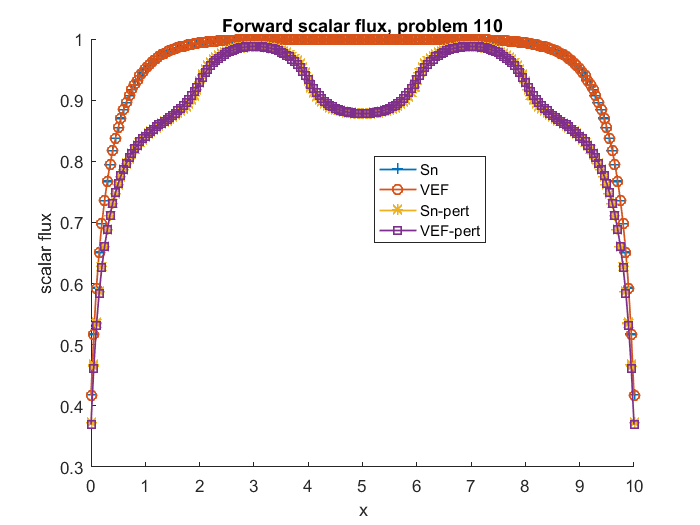
\includegraphics[width=.98\linewidth]{110phi.png}
  \caption{$\phi$ unperturbed and perturbed due to $+15\%$ $\siga$.}
  \label{fig:sfig1}
\end{subfigure}
\begin{subfigure}{.33\textwidth}
  \centering
  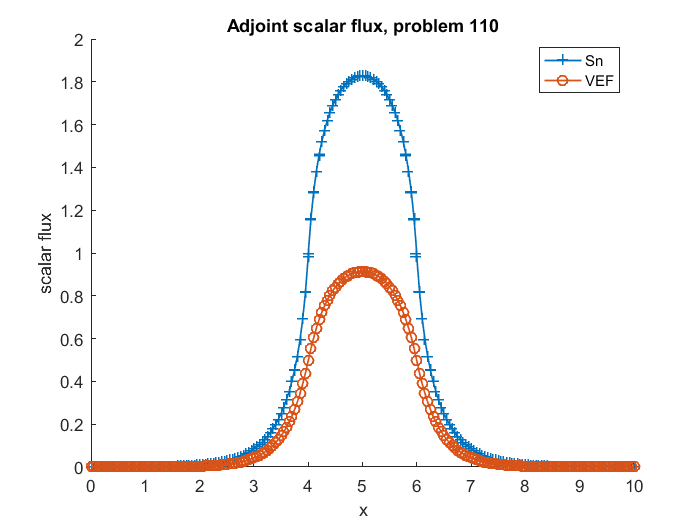
\includegraphics[width=.98\linewidth]{110phia.png}
    \caption{Both Sn and VET adjoints, $\phi^\dag$ and $\varphi^\dag$ respectively.}
  \label{fig:sfig2}
\end{subfigure}%
\begin{subfigure}{.33\textwidth}
  \centering
  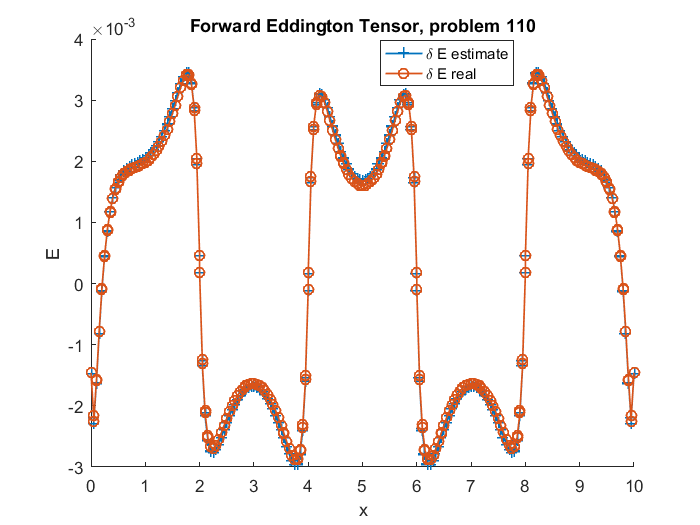
\includegraphics[width=.98\linewidth]{110deltaE.png}
    \caption{Estimation of $\delta \Edd$. Extrapolation point used was $+10\%$ $\siga$.}
  \label{fig:sfig5}
\end{subfigure}%
\label{fig:fig}
\end{figure}		     
		    	\vfill
			    \end{block}
			    \vfill
			    %%%%%%%%%%%%%%%%%%%%%%%%%%%%%%%%%%%%%%%%%%%%%%%%%
			}
			\end{minipage}
		\end{beamercolorbox}
	\end{column}

	%%%%%%%%%%%%%%%%%%%%%%%%%%%%%%%%%%%%%%%%%%%%%%%%%    %%%%%%%%%%%%%%%%%%%%%%%%%%%%%%%%%%%%%%%%%%%%%%%%%
	%%%%%%%%%%%%%%%%%%%%%%%%%%%%%%%%%%%%%%%%%%%%%%%%%
	\begin{column}{.33\textwidth}
		\begin{beamercolorbox}[center,wd=\textwidth]{postercolumn}
			\begin{minipage}[T]{0.95\textwidth} % tweaks the width, makes a new \textwidth
			\parbox[t][\columnheight]{\textwidth}{ % must be some better way to set the the height, width and textwidth simultaneously
			         % Since all columns are the same length, it is all nice and tidy.  You have to get the height empirically

			    %%%%%%%%%%%%%%%%%%%%%%%%%%%%%%%%%%%%%%%%%%%%%%%%%
			    \begin{block}{Eddington estimation continued}

The full sensitivity expression using the estimated $\delta \Edd$ is then

\begin{equation}
\label{SensIP3}
\begin{split}
\delta \qoi =&  \bra \delta q , \varphi^\dag \ket - \bra \delta \isigt \div (\Edd \phi), \grad \varphi^\dag \ket + \bra \delta \sigma_a \phi, \varphi^\dag \ket + \sbra \varphi^\dag, 2 \delta J^{\text{inc}} \sket \\
& - \bra  \isigt \div \left( \delta \Edd \phi \right), \grad \varphi^\dag \ket
- \sbra \varphi^\dag, \phi \delta \BEdd \sket.
\end{split}
\end{equation}			    
			    
Sensitivity for the earlier presented system due to regular perturbations in the source, $\sigs$, and $\siga$. The Sensitivity inner products laid out in Eqs.~\eqref{SensIP1}, ~\eqref{SensIP2}, ~\eqref{SensIP3} are tested against two individual forward solves.
 
\begin{figure}[H]
\label{Case110Sens}
\centering
\begin{subfigure}{.4\textwidth}
  \centering
  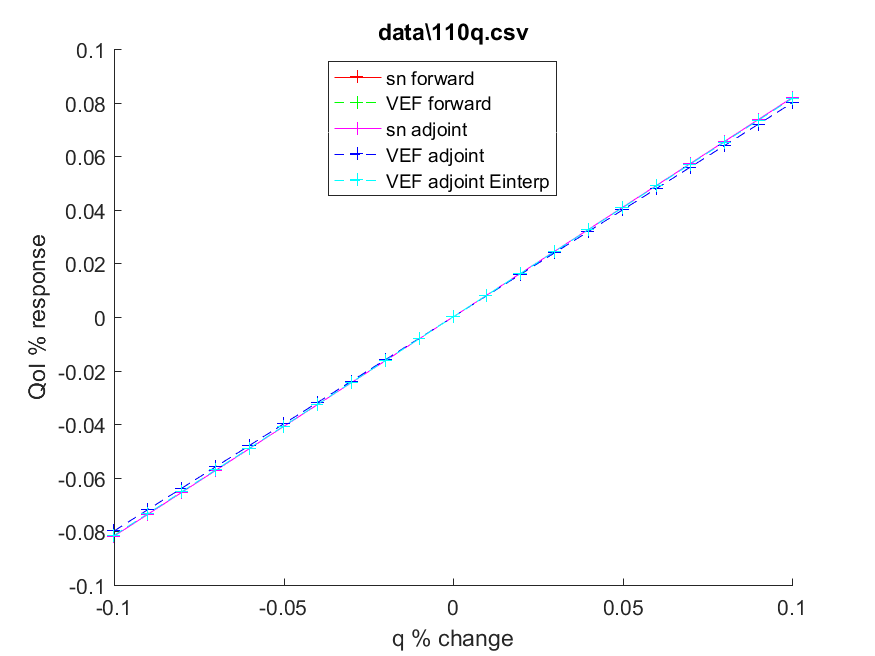
\includegraphics[width=.98\linewidth]{110qSens.png}  \caption{Source sensitivity}
  \label{fig:sfig1}
\end{subfigure}%
\begin{subfigure}{.4\textwidth}
  \centering
  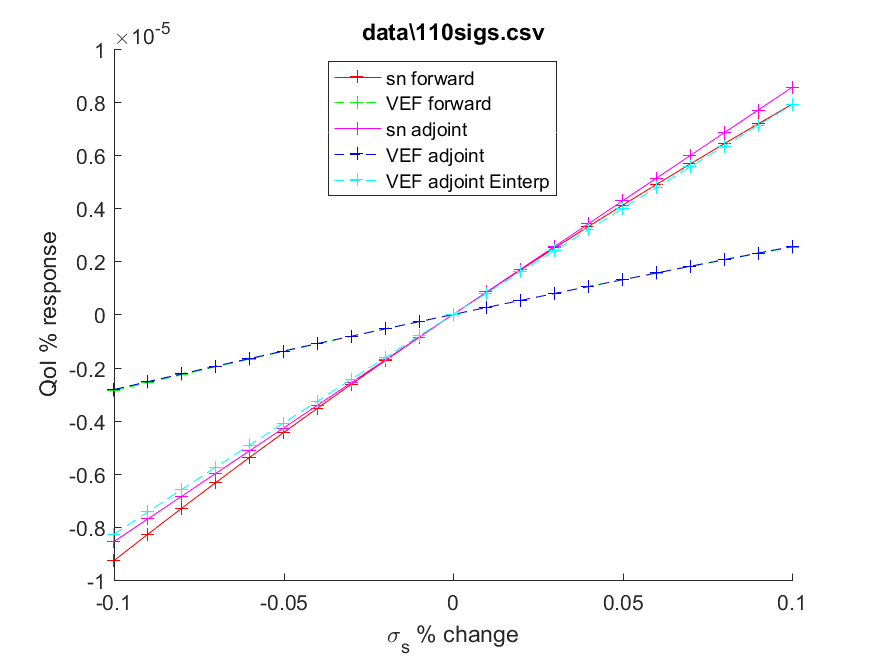
\includegraphics[width=.98\linewidth]{110sigsSens.png}
  \caption{Scattering cross-section sensitivity}
  \label{fig:sfig2}
\end{subfigure}

\begin{subfigure}{.4\textwidth}
  \centering
  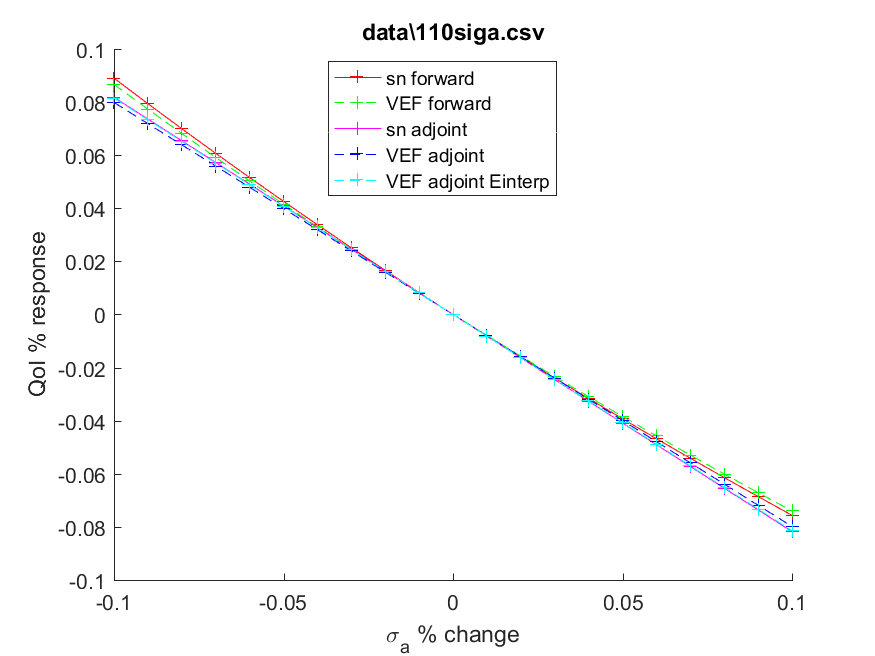
\includegraphics[width=.98\linewidth]{110sigaSens.png}
  \caption{Absorption cross-section sensitivity}
  \label{fig:sfig5}
\end{subfigure}%
\begin{subfigure}{.4\textwidth}
  \centering
  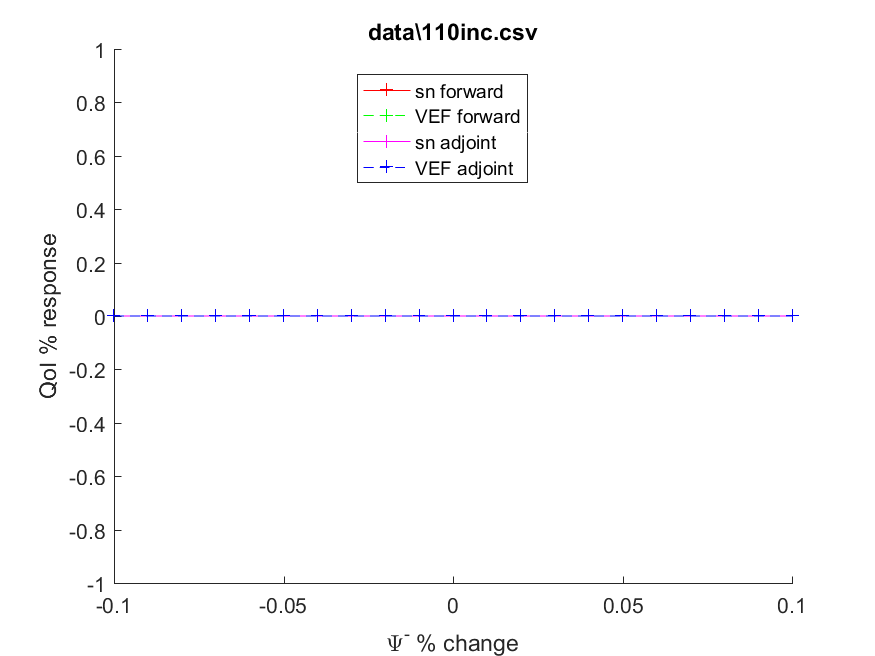
\includegraphics[width=.98\linewidth]{110incSens.png}
  \caption{Incident flux sensitivity}
  \label{fig:sfig4}
\end{subfigure}
\label{fig:fig}
\end{figure}			    
			    
			    
			    \end{block}
			    \vfill
			    %%%%%%%%%%%%%%%%%%%%%%%%%%%%%%%%%%%%%%%%%%%%%%%%%
			    \begin{block}{Conclusion}

$\bullet$ The Eddington formulation of the transport equation yields an adjoint that is not directly related to the Sn transport adjoint.
			    

$\bullet$ This VET adjoint can be used to compute response sensitivity without storing angular flux if assumptions are made about perturbation of the Eddington


$\bullet$ At the additional cost of solving and storing the Sn adjoint scalar flux, exact sensitivity of source perturbations can be obtained, while using VET adjoint for cross-section perturbations

$\bullet$ In situations where numerous perturbation cases must be considered, sampling Eddington values using additional forward solves can increase the VET adjoint accuracy when compared to Sn adjoint. 
			    \end{block}
			    \vfill
			}
			\end{minipage}
		\end{beamercolorbox}
	\end{column}

	\end{columns}
\end{frame}
\end{document}

